%%%%%%%%%%%%%%%%%%%%%%%%%%%%%%%%%%%%%%%%%%%%%%%%%%%%%%%%%%%%%%%%%%%%%%
% How to use writeLaTeX: 
%
% You edit the source code here on the left, and the preview on the
% right shows you the result within a few seconds.
%
% Bookmark this page and share the URL with your co-authors. They can
% edit at the same time!
%
% You can upload figures, bibliographies, custom classes and
% styles using the files menu.
%
%%%%%%%%%%%%%%%%%%%%%%%%%%%%%%%%%%%%%%%%%%%%%%%%%%%%%%%%%%%%%%%%%%%%%%

\documentclass[12pt]{article}
\usepackage{adjustbox}
\usepackage{sbc-template}
\usepackage{todonotes}
\usepackage{graphicx,url}
\usepackage{amsmath}
\usepackage{multirow}
\usepackage[utf8]{inputenc}  
\usepackage{babel}
\usepackage[T1]{fontenc}
\usepackage{xspace}
\usepackage{url}
\usepackage{graphicx}
\usepackage{subfig}
%----------
\usepackage{unicode-math}
\usepackage{babel}
\babeltags{br = brazil, en = english}
\usepackage[T1]{fontenc}
\usepackage{xspace}
\usepackage{url}
%\setmathfont{xits-math.otf}

%\setmathfont[math-style=upright,range={`e,`i}]{xits-math.otf}

%--------------
\sloppy

\title{Calculo Numérico\\Trabalho\_2}


\author{Prof. Dra. Larissa de Freitas \inst{1},\\Guilherme de Souza\inst{1}}

\begin{document} 

\maketitle
\br
%\section{Funções}
%\begin{eqnarray}
%$\lambda x: 5x^{3} - 2x^{2} + 8x - 10$\\
%$\lambda x: 2x^{3} + 5x^{2} + \sin x - 30$\\
%$\lambda x: e^{-x2}\cos x$\\
%    $\lambda x: (x+1)(x-1)(x-3)^{5}\\
%    $\lambda x: (x+2)^{3}\sqrt{x^{2}+1}$
%\end{eqnarray}

\section{Métodos implementados}
\begin{itemize}
  \item Eliminação de Gauss;
  \item Fatoração LU;
  \item Cholesky;
  \item Gauss-Jabobi;
  \item Gauss-Seidel;
  \item Newton.
\end{itemize}

Para execução de tais métodos como, \textbf{Eliminação de Gauss, fatoração LU e Cholesky} foram aplicados na lista de exercícios 6\footnote{Disponivel no AVA:\url{https://ava.ufpel.edu.br/pre/pluginfile.php/313345/mod_resource/content/1/ListaDeExercicios6.pdf}}. Os métodos de \textbf{Gauss-Jacobi} e \textbf{Gauss-Seidel} utilizou-se a lista de exercícios 5\footnote{Disponivel no AVA:\url{https://ava.ufpel.edu.br/pre/pluginfile.php/312500/mod_resource/content/1/ListaDeExercicios5.pdf}}. E por ultimo na lista de exercício 7\footnote{Disponivel no AVA:\url{https://ava.ufpel.edu.br/pre/pluginfile.php/313753/mod_resource/content/1/ListaDeExercicios7.pdf}}.


\section{Eliminação de Gauss}
%---------------------------------------------------------------------------------------------------
% MATRIZ NUMERO 1
%---------------------------------------------------------------------------------------------------
\begin{table}[htb]
  \begin{minipage}[b]{.46\linewidth}

    \centering
    \begin{tabular}{|c c c|c|}
        -2           &          3           &          1      &   -5 \\
        2           &          1           &          -4      &   -9 \\
        7           &          10           &          -6     &   2 \\
    \end{tabular}
    \caption{Matriz de entrada 1}
    \label{tab:esq}

  \end{minipage}\hfill
  \begin{minipage}[b]{.46\linewidth}

    \centering
    \begin{tabular}{|c c c|c|}
        7           &          10           &          -6      &   2 \\
        0           &          5           &          0      &   -4 \\
        0           &          0           &          -2     &   -9 \\
    \end{tabular}
    \caption{Matriz resultante 1}
    \label{tab:dir}
  \end{minipage}
\end{table}


\begin{table}[!h]
\centering
\begin{tabular}{|l|}
\multicolumn{1}{|c|}{5.2857} \\
-0.8                         \\
4.5                         
\end{tabular}
\caption{Resultado matriz 1}
\end{table}

%---------------------------------------------------------------------------------------------------
% MATRIZ DOIS
%---------------------------------------------------------------------------------------------------

\begin{table}[htb]
  \begin{minipage}[b]{.46\linewidth}

    \centering
    \begin{tabular}{|c c c c|c|}
        1           &         -3          &           5     &   6     &   17\\
        -9          &         4           &          -1     &   0     &   29\\
        3           &         2           &          -2     &   7     &   -11\\
        1           &         2           &           5     &   -4    &   7\\
    \end{tabular}
    \caption{Matriz de entrada 2}
    \label{tab:esq}

  \end{minipage}\hfill
  \begin{minipage}[b]{.46\linewidth}

    \centering
    \begin{tabular}{|c c c c|c|}
        -9           &         4          &           -1     &   0     &   29\\
        0          &         3           &          -2     &   7     &   -1\\
        0           &         0           &          5     &   -8     &   10\\
        0           &         0           &           0     &   13    &   15\\
    \end{tabular}
    \caption{Matriz resultante 2}
    \label{tab:dir}
  \end{minipage}
\end{table}


\begin{table}[!h]
\centering
\begin{tabular}{|l|}
\multicolumn{1}{|c|}{-3.8547} \\
-0.4615                         \\
3.8462                        \\
1.1538
\end{tabular}
\caption{Resultado matriz 2}
\end{table}

%---------------------------------------------------------------------------------------------------
% MATRIZ 3
%---------------------------------------------------------------------------------------------------
\begin{table}[htb]
  \begin{minipage}[b]{.46\linewidth}

    \centering
    \begin{tabular}{|c c c c|c|}
        -2           &         3          &           1     &   5     &   2\\
        5          &         1           &          -1     &   0     &   -1\\
        1           &         6           &          3     &   -1     &   0\\
        4          &         5           &           2     &   8    &   6\\
    \end{tabular}
    \caption{Matriz de entrada 3}
    \label{tab:esq}

  \end{minipage}\hfill
  \begin{minipage}[b]{.46\linewidth}

    \centering
    \begin{tabular}{|c c c c|c|}
        5           &         1          &           -1     &   0     &   -1\\
        0          &         5           &          3     &   -1     &   0\\
        0           &         0           &          -1     &   5     &   1\\
        0           &         0           &           0     &   8    &   6\\
    \end{tabular}
    \caption{Matriz resultante 3}
    \label{tab:dir}
  \end{minipage}
\end{table}


\begin{table}[!h]
\centering
\begin{tabular}{|l|}
\multicolumn{1}{|c|}{0.65} \\
-1.5                         \\
3.75                        \\
0.75
\end{tabular}
\caption{Resultado matriz 3}
\end{table}

%---------------------------------------------------------------------------------------------------
% MATRIZ 4
%---------------------------------------------------------------------------------------------------
\begin{table}[htb]
  \begin{minipage}[b]{.46\linewidth}

    \centering
    \begin{tabular}{|c c c c c|c|}
        0           &         1          &           3     &   2     &   4   &   3\\
        8          &         -2           &          9     &   -1     &   2   &   -5\\
        5           &         1           &          1     &   7     &   2   &   6\\
        -2          &         4           &           5     &   1    &     0   &   -1\\
        7          &         -3           &           2     &   -4    &     1   &   8\\
    \end{tabular}
    \caption{Matriz de entrada 4}
    \label{tab:esq}

  \end{minipage}\hfill
  \begin{minipage}[b]{.46\linewidth}

    \centering
    \begin{tabular}{|c c c c c|c|}
        8           &         -2          &           9     &   -1     &   2   &   -5\\
        0          &         3           &          7     &   0     &   0   &   -2\\
        0           &         0           &          -8     &   7     &   0   &   10\\
        0          &         0           &           0     &   -4    &     0   &   8\\
        0          &         0           &           0     &   0    &     4   &   7\\
    \end{tabular}
    \caption{Matriz resultante 4}
    \label{tab:dir}
  \end{minipage}
\end{table}


\begin{table}[!h]
\centering
\begin{tabular}{|l|}
\multicolumn{1}{|c|}{3.6458} \\
6.3333                         \\
-3                        \\
-2                        \\
1.75
\end{tabular}
\caption{Resultado matriz 4}
\end{table}


\section{Fatoração LU}


%---------------------------------------------------------------------------------------------------
% MATRIZ 1
%---------------------------------------------------------------------------------------------------
\begin{table}[htb]
  \begin{minipage}[b]{.46\linewidth}

    \centering
    \begin{tabular}{|c c c|c|}
        1           &         0          &           0     &   0\\
        0.25           &         1          &           0     &   0\\
        1.25           &         1          &           1     &   0\\
        0.5           &         0.6667          &           1     &   1\\
    \end{tabular}
    \caption{Matriz LU 1}
    \label{tab:dir}

  \end{minipage}\hfill
  \begin{minipage}[b]{.46\linewidth}

    \centering
    \begin{tabular}{|c c c|c|}
        4           &         -1          &           3     &   8\\
        0           &         6          &           1     &   -5\\
        0           &         0          &           -3     &   -5\\
        0           &         0          &           0     &   5\\
    \end{tabular}
    \caption{Matriz U 1}
    \label{tab:esq}

  \end{minipage}\hfill
  \begin{minipage}[b]{.46\linewidth}

    \centering
    \begin{tabular}{|c|}
        -3\\
        4\\
        4\\
        6\\
    \end{tabular}
    \caption{Resolução Matriz 1}
    \label{tab:dir}
  \end{minipage}
\end{table}


%---------------------------------------------------------------------------------------------------
% MATRIZ 2
%---------------------------------------------------------------------------------------------------
\begin{table}[htb]
  \begin{minipage}[b]{.36\linewidth}

    \centering
    \begin{tabular}{|c c c c c|}
        1                 &         0                   &           0             &   0     &   0   \\
        -0.33333          &         1                   &          0               &   0     &   0   \\
        2.66667           &         27.99946           &          1                &   0     &   0   \\
        0.66667          &         -4.99988           &           -0.21978          &   1    &     0  \\
        -0.33333          &         6.99988           &           0.26027           &   0.17222    &     1\\
    \end{tabular}
    \caption{Matriz LU 2}
    \label{tab:dir}


  \end{minipage}\hfill
  \begin{minipage}[b]{.46\linewidth}

    \centering
    \begin{tabular}{|c|}
        -68\\
        28\\
        280\\
        -72\\
        362\\
    \end{tabular}
    \caption{Resolução Matriz 1}
    \label{tab:dir}
  \end{minipage}\hfill
  \begin{minipage}[b]{.36\linewidth}

    \centering
    \begin{tabular}{|c c c c c|}
        3                 &         -2       &           -1             &   7     &   3   \\
        0          &         0.33334          &          2.66667        &   0.33331     &   -2.00001   \\
        0           &         0               &          -72.99865      &   -27.99919     &   49.99919   \\
        0          &         0                &           0             &   -4.13704    &     -1.041\\
        0          &         0                &           0             &   0    &     0.16581\\
    \end{tabular}
      \caption{Matriz U 2}
    \label{tab:esq}
  \end{minipage}

\end{table}

%---------------------------------------------------------------------------------------------------
% MATRIZ 3
%---------------------------------------------------------------------------------------------------

\begin{table}[htb]
  \begin{minipage}[b]{.46\linewidth}

    \centering
    \begin{tabular}{|c c c c c c|}
        1           &         0          &           0                        &   0             &   0      &   0\\
        0.25          &         1           &          0                      &   0             &   0      &   0\\
        -0.5           &         -1.66666667           &          1           &   0             &   0     &   0\\
        1.75           &         4           &           -2.03743315          &   1             &   0       &   0\\
        2.5           &         3.83333333           &           -2.133636363 &   0.27928898    &   1       &   0\\
        2           &         2.33333333           &           -1.53475936    &   0.6587665    &   -1.9408528       &   1\\
    \end{tabular}
    \caption{Matriz L 3}
    \label{tab:esq}

  \end{minipage}\hfill
  \begin{minipage}[b]{.46\linewidth}

    \centering
    \begin{tabular}{|c c c c c c|}
        4           &         12          &           14                        &   5             &   2      &   -1\\
        0          &         -6           &          8.5                      &   0.75             &   2.5      &   -1.75\\
        0           &       0           &          31.1666667           &   4.75             &   3.166666666     &   -3.41666667\\
        0           &         0           &           0          &   9.92780746             &   0.95187167       &   11.78877006\\
        0           &         0           &           0 &   0    &   3.91597093       &   -9.38338265\\
        0           &       0           &           0    &   0    &   0       &   -10.1382391\\
    \end{tabular}
    \caption{Matriz U 3}
    \label{tab:dir}
  \end{minipage}\hfill

  \begin{minipage}[b]{.46\linewidth}

    \centering
    \begin{tabular}{|c|}
        23\\
        11\\
        14\\
        -80\\
        66\\
        41\\
    \end{tabular}
    \caption{Resolução Matriz 1}
    \label{tab:dir}
  \end{minipage}\hfill
\end{table}

\section{Gráficos}
Nesta seção, será apresentado os gráficos gerados a partir da função aplicada aos métodos aqui apresentados e aprendido em aula. Para uma melhor comparação, os gráficos estão dispostos da mesma forma que as tabelas, cada método com a mesma função de entrada. Desta forma a comparação visual é facilitada.

\begin{figure}[!h]
    \centering
    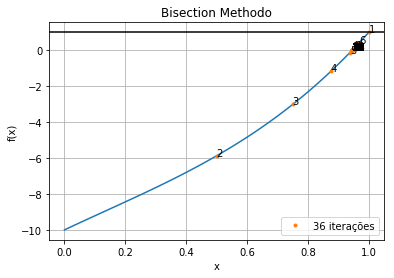
\includegraphics[scale=0.5]{/home/souza/Documents/semestre_2019-2/calculo_numerico/trabalho_1/graficos/bisection_f1.png}
    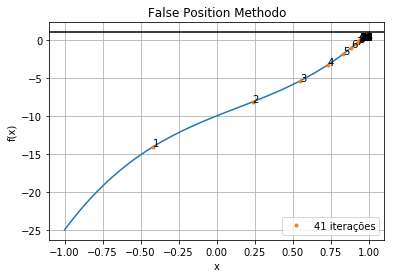
\includegraphics[scale=0.5]{/home/souza/Documents/semestre_2019-2/calculo_numerico/trabalho_1/graficos/false_position_f1.png}\\
    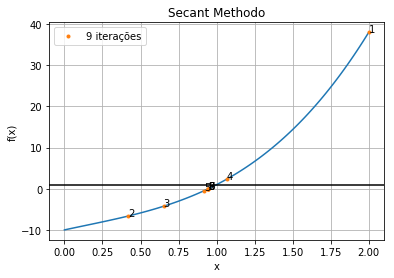
\includegraphics[scale=0.5]{/home/souza/Documents/semestre_2019-2/calculo_numerico/trabalho_1/graficos/secant_f1.png}
    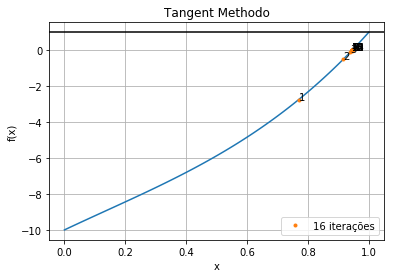
\includegraphics[scale=0.5]{/home/souza/Documents/semestre_2019-2/calculo_numerico/trabalho_1/graficos/tangent_f1.png}
    \caption{Gráficos da função um executada pelos quatro métodos presentes.}
\end{figure}

\begin{figure}[!h]
    \centering
    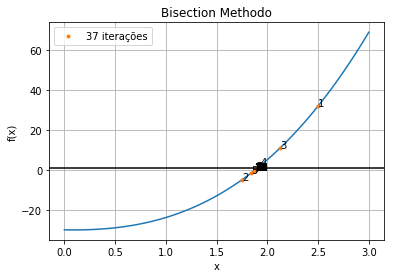
\includegraphics[scale=0.5]{/home/souza/Documents/semestre_2019-2/calculo_numerico/trabalho_1/graficos/bisection_f2.png}
    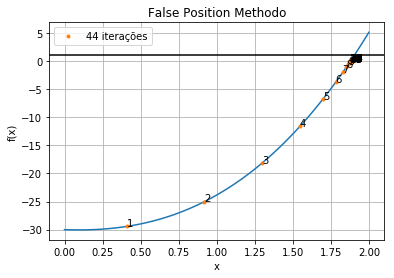
\includegraphics[scale=0.5]{/home/souza/Documents/semestre_2019-2/calculo_numerico/trabalho_1/graficos/false_position_f2.png}\\
    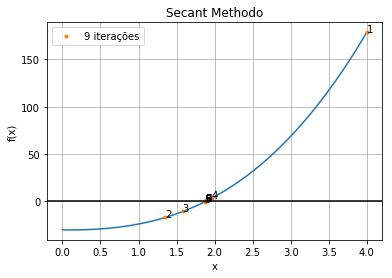
\includegraphics[scale=0.5]{/home/souza/Documents/semestre_2019-2/calculo_numerico/trabalho_1/graficos/secant_f2.png}
    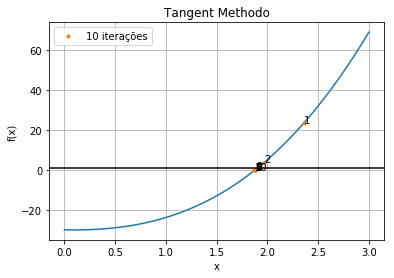
\includegraphics[scale=0.5]{/home/souza/Documents/semestre_2019-2/calculo_numerico/trabalho_1/graficos/tangent_f2.png}
    \caption{Gráficos da função dois executada pelos quatro métodos presentes.}
\end{figure}

\begin{figure}[!h]
    \centering
    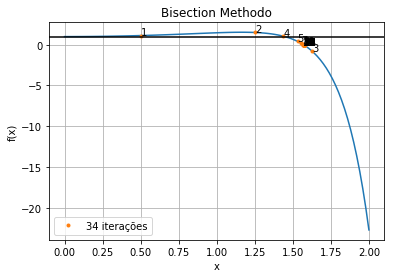
\includegraphics[scale=0.5]{/home/souza/Documents/semestre_2019-2/calculo_numerico/trabalho_1/graficos/bisection_f3.png}
    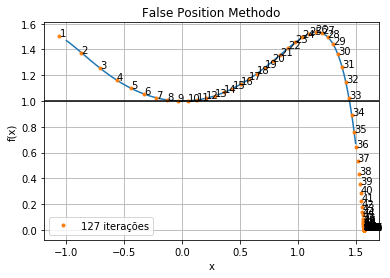
\includegraphics[scale=0.5]{/home/souza/Documents/semestre_2019-2/calculo_numerico/trabalho_1/graficos/false_position_f3.png}\\
    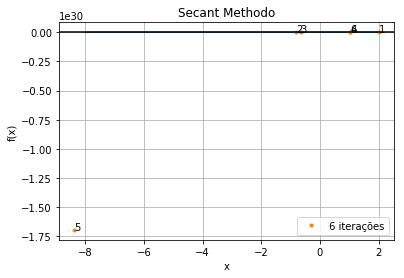
\includegraphics[scale=0.5]{/home/souza/Documents/semestre_2019-2/calculo_numerico/trabalho_1/graficos/secant_f3.png}
    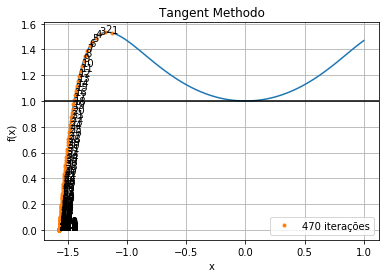
\includegraphics[scale=0.5]{/home/souza/Documents/semestre_2019-2/calculo_numerico/trabalho_1/graficos/tangent_f3.png}
    \caption{Gráficos da função três executada pelos quatro métodos presentes.}
\end{figure}

\begin{figure}[!h]
    \centering
    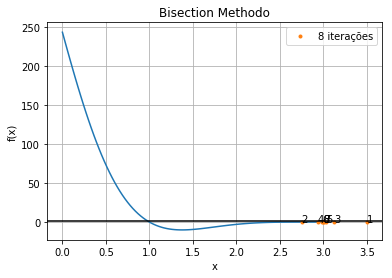
\includegraphics[scale=0.5]{/home/souza/Documents/semestre_2019-2/calculo_numerico/trabalho_1/graficos/bisection_f4.png}
    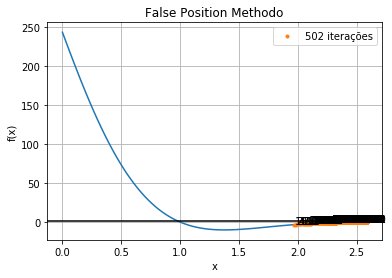
\includegraphics[scale=0.5]{/home/souza/Documents/semestre_2019-2/calculo_numerico/trabalho_1/graficos/false_position_f4.png}\\
    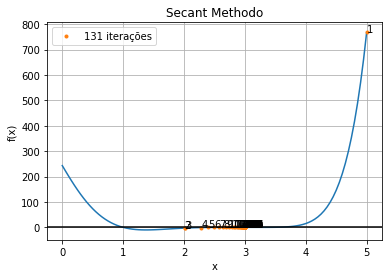
\includegraphics[scale=0.5]{/home/souza/Documents/semestre_2019-2/calculo_numerico/trabalho_1/graficos/secant_f4.png}
    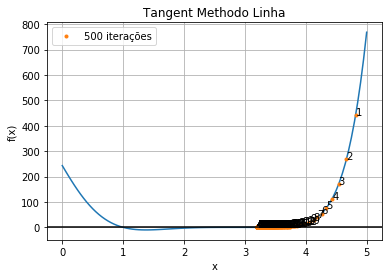
\includegraphics[scale=0.5]{/home/souza/Documents/semestre_2019-2/calculo_numerico/trabalho_1/graficos/tangent_f4.png}
    \caption{Gráficos da função quatro executada pelos quatro métodos presentes.}
\end{figure}

\begin{figure}[!h]
    \centering
    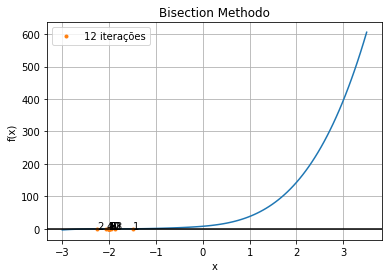
\includegraphics[scale=0.5]{/home/souza/Documents/semestre_2019-2/calculo_numerico/trabalho_1/graficos/bisection_f5.png}
    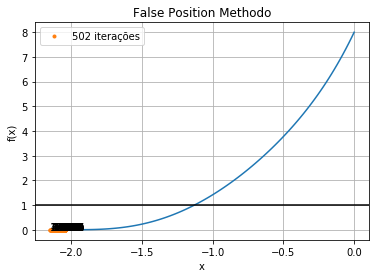
\includegraphics[scale=0.5]{/home/souza/Documents/semestre_2019-2/calculo_numerico/trabalho_1/graficos/false_position_f5.png}\\
    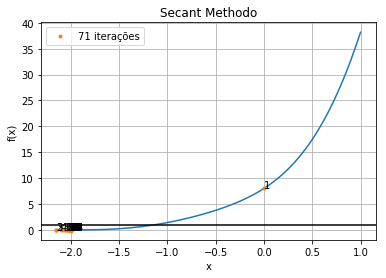
\includegraphics[scale=0.5]{/home/souza/Documents/semestre_2019-2/calculo_numerico/trabalho_1/graficos/secant_f5.png}
    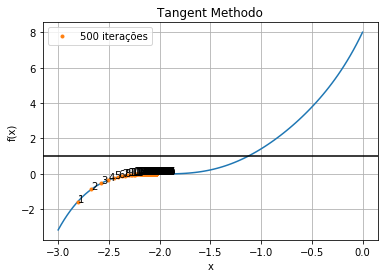
\includegraphics[scale=0.5]{/home/souza/Documents/semestre_2019-2/calculo_numerico/trabalho_1/graficos/tangent_f5.png}
    \caption{Gráficos da função cinco executada pelos quatro métodos presentes.}
\end{figure}
\end{document}
